\chapter{RESULTADOS E DISCUSSÃO}

Entender como a contribuição acadêmica influencia na intenção inicial da carreira empreendedora bem-sucedida é de grande interesse para centros acadêmicos, profissionais e educadores em empreendedorismo. 
Desta forma o resultados desta pesquisa encontram-se divididos em seções, que atendem aos objetivos propostos no estudo. 

Inicialmente serão apresentadas descrições que caracterizam os dois perfis estudados (pré-programa  e pós-programa) em relação às variáveis e as comparações entre os grupos.
Posteriormente serão apresentadas as inovações produzidas pelos alunos participantes durante o percurso do programa.

\section{Alcance da amostra}

Para o desenvolvimento do programa foi alcançado 26 equipes apresentando ao todo 118 alunos oriundos dos cursos do centro de agrárias e mais outras áreas: \textit{Artes Visuais}, \textit{Administração}, \textit{Design Gráfico}, \textit{Engenharia Química}, \textit{Engenharia de Produção}, \textit{Marketing e Ecologia}. 

Os dados coletados revelam que, nas 115 respostas válidas que compõem a amostra à faixa etária no período de inscrição, apresentavam 75,4\% dos estudantes possuíam idade menor que 20 anos, 16,1\% apresentaram a intervalo de idades entre 21 e 25 anos, e 59\% tinham idade maior que 25 anos.


\begin{table}[!htb]
\centering
\caption{\textbf{Faixa etária dos alunos inscritos no programa}}
\label{tab:tabela_4}
\begin{tabular}{clccc}
\hline \hline
{\textbf{Dados}} & {\color[HTML]{000000} \textbf{Faixa etária}} & \multicolumn{3}{c}{{\color[HTML]{000000} \textbf{Inscritos}}} \\ \cline{1-5}
{\color[HTML]{000000} } & {\color[HTML]{000000} } & \multicolumn{1}{l}{{\color[HTML]{000000} \textbf{Frequência (\%)}}} & \multicolumn{1}{l}{{\color[HTML]{000000} \textbf{Porcentagem (\%)}}} & \multicolumn{1}{l}{{\color[HTML]{000000} \textbf{Válidos (\%)}}} \\
{\color[HTML]{000000} } & {\color[HTML]{000000} \textbf{Menor que 20}} & {\color[HTML]{000000} 89} & {\color[HTML]{000000} 75,4} & {\color[HTML]{000000} 77,4}\\[8pt]
\multirow{-3}{*}{{\color[HTML]{000000} \textbf{}}} & {\color[HTML]{000000} \textbf{De 21 a 25}} & {\color[HTML]{000000} 19} & {\color[HTML]{000000} 16,1} & {\color[HTML]{000000} 16,5} \\[8pt]
\multicolumn{1}{l}{{\color[HTML]{000000} \textbf{Válidos}}} & {\color[HTML]{000000} \textbf{Maior que 25}} & {\color[HTML]{000000} 7} & {\color[HTML]{000000} 5,9} & {\color[HTML]{000000} 6,1}\\[8pt]
\multicolumn{1}{l}{{\color[HTML]{000000} \textbf{}}} & {\color[HTML]{000000} \textbf{Total}} & {\color[HTML]{000000} 115} & {\color[HTML]{000000} 97,5} & {\color[HTML]{000000} } \\[8pt]\hline
\multicolumn{1}{l}{{\color[HTML]{000000} \textbf{Omissos}}} & {\color[HTML]{000000} \textbf{Não informou}} & {\color[HTML]{000000} 3} & {\color[HTML]{000000} 2,5} & {\color[HTML]{000000} } \\[8pt] \hline
\multicolumn{2}{c}{{\color[HTML]{000000} \textbf{TOTAL GERAL}}} & {\color[HTML]{000000} 118} & {\color[HTML]{000000} } & {\color[HTML]{000000} } \\ \hline\hline
\end{tabular}
\fonte{Autoria própria}
\end{table}

O curso que mais apresentou inscrições dos alunos foi o de Engenharia Agronômica, representando 47,32\% deste total, enquanto os cursos de Engenharia Agrícola, Zootecnia, Engenharia de Pesca e Engenharia Florestal tiveram participações consideravelmente menores, com apenas 11,61\%, 19,64\%, 4,46\% e 6,25\% dos estudantes inscritos, respectivamente, já o curso de Medicina veterinária não apresentou alunos inscritos. Na figura  \ref{figura_10} é possível observar a quantidade de alunos inscritos e seus respectivos cursos.

\begin{figure}[!htb]
\caption{\textbf{Porcentagem de alunos inscritos no programa por curso}}
\centering
\includegraphics[scale=0.3]{Imagens/inscritos.png}
\fonte{Autoria própria}
\label{figura_10}
\end{figure}



\section{Áreas e cadeias produtivas}

A fase inicial do programa alcançou 27 propostas de protótipos e/ou negócios na área rural com foco na agricultura sustentável. Na figura \ref{figura_11} é possível verificar as áreas e cadeias produtivas prioritárias escolhidas.

\begin{figure}[!htb]
\centering
\caption{\textbf{Áreas e potenciais propostas de negócios escritos}}
\includegraphics[scale=0.3]{Imagens/propostas_negocios.png}
\fonte{Autoria própria}
\label{figura_11}
\end{figure}
\newpage




\section{Contextualizando o cenário da prática}

Primeiramente, foi criado um site \href{http://www.empreendaagrosustentavel.com}{empreendaagroustentavel.com} para divulgação do programa proposto, bem como a inclusão de materiais sobre os assuntos abordados durante todo o programa, textos de interesse,link para o canal de podcasts \href{https://open.spotify.com/show/3c25hRSxvaCFPw6Y3lX3i1?si=9H_fGz_uRgGiFNhAcdr4rQ}{Empreenda AGROCAST}.





Os encontros com os alunos aconteceram mensalmente, de maneira presencial durante dois dias em dois turnos. A proposta da metodologia contemplou a divulgação semanal de atividades desenvolvidas pelos grupos, afim de manter o engajamento dos participantes e desenvolvimento das propostas de negócios pensadas ao entrarem no programa. 

A cada workshop, foram desenvolvidas atividades práticas, obedecendo aos seguintes critérios: 
Desenvolvimento gradual do ideia de negócio de forma planejada; Desenvolvimento de planos de negócios e planos gerenciais; Desenvolvimento do mínimo produto economicamente viável; Aprendizado e estratégia de apresentação do produto proposto. O indivíduo é o conjunto de seus Conhecimentos, Habilidades e Atitudes (CHA) \cite{dutra_competencias:_2004}, conjunto este de grande relevância para um empreendedor, especialmente porque as competências se mostram como parte fundamental da formação do empreendedor nos dias atuais, o qual assume a responsabilidade de agregar valor às organizações \cite{ferreira_conhecimento_2019}, desta forma, o se mostra importante o aprendizado contínuo e multidisciplinar para fixação e melhor desenvolvimento do aprendizado. Quando o aprendizado ocorre por meio de metodologias ativas, o conhecimento dos estudantes é comparável ao do método tradicional, porém, seu desempenho em relação às suas habilidades e atitudes é superior, reflexo da visão crítico reflexiva proporcionada pelo método \cite{limberger_metodologias_2013}.

Foram executados quatro workshops, nos quais foram abordados conceitos de empreendedorismo, ideação, modelo de negócios, marketing, entre outros. As oficinas foram conduzidas através de palestras, atividades práticas e dinâmicas, ou seja, metodologias ativas. Os workshops foram conduzidos no formato de “Jornada” (Figura \ref{figura_17}), ou seja, os participantes foram apresentados gradativamente a conteúdos e metodologias. 







\begin{figure}[!htb]
\centering
\caption{\textbf{Jornada Empreenda Agro Sustentável}}
\includegraphics[scale=0.4]{Imagens/jornada.png}
\fonte{Próprio Autor}
\label{figura_17}
\end{figure}

O primeiro Workshop teve como foco o desenvolvimento de palestras e oficinas que abordaram temas relacionados ao empreendedorismo, tais como: \textbf{Startups (O que é, o que come, onde vive??)}, \textbf{Empreendedorismo, comportamento empreendedor e cultura empreendedora},  \textbf{Problemas (segmentação do mercado)}, segundo as ODS, entre outros.  



\begin{figure}[!h]
\center
\caption{\textbf{1º Workshop Empreenda Agro Sustentável}}
\subfigure[ref1][Participantes do programa: 1º dia ]{\includegraphics[scale=0.15]{Imagens/primeiro_dia_1.jpg}}
\qquad
\subfigure[ref2][Participantes do programa: 2º dia]{\includegraphics[scale=0.15]{Imagens/primeiro_dia_2.jpg}}
\qquad
\subfigure[ref3][Participantes do programa: 2º dia]{\includegraphics[scale=0.15]{Imagens/primeiro_dia_3.jpg}}
\qquad
\subfigure[ref4][Participantes do programa: 2º dia]{\includegraphics[scale=0.15]{Imagens/primeiro_dia_4.jpg}}
\fonte{Próprio Autor}.
\label{figura_29}
\end{figure}
\newpage



\section{Tratamento dos grupos de itens: Autoeficácia, Intenção empreendedora, Apoio Familiar}

O método de rotação Varimax com normalização de Kaiser\footnotemark[1] apresentou 3 componentes principais para esta pesquisa, aglutinando as questões na ordem apresentada na tabela \ref{tabela_3}:


\begin{longtable}[!h]{p{6cm} c c c }
\caption{\textbf{Estrutura fatorial da medida de intenção empreendedora}}
\label{tabela_3}\\
\hline \hline


\multicolumn{1}{p{6cm}}{} & \multicolumn{3}{c}{\textbf{Fatores}}\\ 
 \multicolumn{1}{c}{\textbf{Itens}} & \multicolumn{3}{c}{\hrulefill}\\ 

 \multicolumn{1}{c}{} 
 &\multicolumn{1}{p{1.5cm}}{\textbf{Autoeficácia}} & \multicolumn{1}{p{1.5cm}}{\textbf{Intenção}} &\multicolumn{1}{p{1.5cm}}{\textbf{Família}}  
\\ \hline 

\endfirsthead


\multicolumn{4}{l}{{{\bfseries \tablename \ \thetable{} -\ \textbf{Estrutura fatorial da medida de intenção empreendedora}}}}\\
\multicolumn{4}{r}{\bfseries \textbf{(continuação)}}\\

\hline \multicolumn{1}{p{6cm}}{\textbf{Questões}} &\multicolumn{1}{c}{\textbf{Autoeficácia}} & \multicolumn{1}{c}{\textbf{Intenção}} &\multicolumn{1}{c}{\textbf{Família}}  
\\ \hline 

\endhead

\hline \multicolumn{4}{r}{\textbf{(Continua)}} \\ \hline


\endfoot
\hline \multicolumn{4}{r}{\textbf{(Conclusão)}} \\ \hline
\hline \hline

\endlastfoot


Estabelecer e atingir metas e objetivos
 &  ,752 & & \\\\
 
Gerar novas ideias
 &  ,702 & & \\\\
 
Desenvolver novos produtos
 &  ,772 & & \\\\
 
Fazer análises financeiras
 &  ,547 & & \\\\
 
Reduzir riscos e incertezas
 &  ,683 &  & \\\\
 
Assumir riscos calculados
 &   ,463 & \textbf{,451} & \\\\
 
Tomar decisões em situações de risco
 &   ,522 & & \\\\
 
Administrar o tempo estabelecendo metas
 &   ,649 & & \\\\
 
Responsabilizar-me por ideias e decisões
 & ,456 & &  \\\\
 
Começar minha própria empresa
& ,603 & \textbf{,435}  & \\\\

Conduzir minha própria empresa ao sucesso
 & ,658 & \textbf{,470}  & \\\\
Eu já sou meu próprio patrão na empresa que eu fundei
 & & ,430 &  \\\\

Para mim, ser um empreendedor implica em mais vantagens do que desvantagens
 &  & ,727  & \\\\
 
Uma carreira como empreendedor é atrativa
 &  & ,890  & \\\\
 
Se tivesse a oportunidade e os recursos, eu me tornaria um empreendedor
 &  & ,788 & \\\\
 
Ser um empreendedor traria grande satisfação
 &  & ,821 & \\\\
 
Por gentileza, indique se você tem pensado e o quão seriamente tem pensado em criar seu próprio negócio
 &  & ,588 & \\\\
 
O capital oferecido por minha família e empréstimo em condições flexíveis são facilitadas
 &  & & ,618 \\\\
 
Minha família me fornece contatos com pessoas que podem me ajudar na carreira de empreendedor
 &  & & ,658 \\\\
 
Minha família me apresenta pessoas de sua rede de relação de negócios
 &  & & ,400 \\\\
 
Minha família me transmite conhecimentos ligados ao meu setor de atividade
 &  & & ,618 \\\\
 
Meus pais / minha família são meus mentores ou \textit{coachs} nas minhas atividades de empreendedor
 &  & & ,687 \\\\
 
Minha família me fornece locais/ infraestrutura para minhas atividades de empreendedor.
 &  & & ,658 \\\\
 
Meus pais ou família me concedem acesso a uma rede de distribuição para minha empresa.
 &  & & ,702 \\\\
 
 
Minha família me empresta capital que  tenho que pagar regularmente a eles com juros		
 &  & & ,583 \\\\
 
Minha família me empresta capital sem a necessidade de juros e que pode ser perdido se o negócio falir
 & & & ,556 \\\\ \hline 
 
\end{longtable}
\fonte{Autoria própria}
\footnotetext[1]{Método de Extração: Análise de Componente Principal.\\Método de Rotação: Varimax com Normalização de Kaiser.}



\begin{table}[!htb]
 \label{tabela_4}
 \centering
\caption{\textbf{Variância total explicada}}
 \\ \hline\hline
\begin{tabular}{c c c c }
\multicolumn{1}{p{6cm}}{} & \multicolumn{3}{c}{\textbf{Fatores}}\\ 
 \multicolumn{1}{c}{\textbf{Itens}} & \multicolumn{3}{c}{\hrulefill}\\ 

 \multicolumn{1}{c}{} 
 &\multicolumn{1}{c}{\textbf{Autoeficácia}} & \multicolumn{1}{c}{\textbf{Intenção}} &\multicolumn{1}{c}{\textbf{Família}}  
\\\\ \hline 

 Somas de rotação de carregamentos ao quadrado (n)
 & 6,602 & 4,090 & 2,802 \\\\
 Variância explicada (\%)
 & 22,766 & 14,102 & 9,662\\\\
 Variância cumulativa (\%)
 & 22,766\% & 36,868\% & 46,530\% \\\hline \hline 
 
\end{tabular}
\fonte{Adaptado de \cite{lima_sauglobal_2017}}.
\end{table}



As questões: \textbf{"Para mim sem empresa não é autônomo"} e \textbf{"Pensando em todos os possíveis recursos que minha família me fornece, eu sou completamente independente dela para decidir como alocá-los e usá-los.			
"}, foram eliminadas da pesquisa, pois foi adotado a supressão de coeficientes que apresentaram valores absolutos a baixo de 0,40, já as questões: \textbf{Assumir riscos calculados}, \textbf{Conduzir minha própria empresa ao sucesso} e \textbf{Começar minha própria empresa}, apresentaram valores satisfatórios tanto para dimensão Autoeficácia quanto para dimensão intenção empreendedora, porem foi considerado o valor de coeficiente mais alto.



\section{Resultado Dimensão autoeficácia empreendedora}


Considerando que os escores das perguntas relacionadas a dimensão empreendedora variam de
1, menor número, a 7, maior número na escala,
foi avaliada a média de cada variável (questão),
o histograma (Figura \ref{figura_29}), foi extraído partindo da medina de cada resposta aglutinadas em fatores, onde quanto mais próximo de 7, melhor a perspectiva de mudança positiva para a amostra pesquisada que se inscreveu e participou do programa. Foi observado utilizando o Teste-t pareado com o intervalo de confiança em 95\%  que a autoeficácia para os participantes, sem levar em consideração as diferenças dos cursos, não variou significativamente (p-value 0,118), porem, observando as médias nos histogramas das respostas antes e após a participação do programa passou de 5,31 (Figura \ref{figura_29}a) para 5,65 (Figura \ref{figura_29}b) e que as respostas aumentaram a frequência para os quesitos 6 \textit{"Seguro"} e \textit{7"Completamente seguro"}.

A autoeficácia empreendedora é uma importante dimensão para a geração de inovação e criatividade para novos negócios e produtos escaláveis. Neste sentido, as instituições de ensino superior, independente da ciência de estudo deve ser capaz de proporcionar atividades didáticas que tenham como propósito a melhoria do nível da autoeficácia dos alunos resultando numa melhora das competências empreendedoras  pós formação dos mesmos \cite{ribeiro_autoeficacia_2019}. A busca pela melhoria da dimensão da autoeficácia empreendedora ajudará a moldar o futuro dos alunos no mercado de trabalho e motivará a ter sucesso em seus futuros negócios, permitindo assim os alunos  definir e seguir o seu próprio percurso profissional com sucesso  \cite{das_examining_2018}.

\begin{figure}[!h]
\center
\caption{\textbf{Dimensão da autoeficácia empreendedora para os cursos de agrárias após a participação do programa}}
\subfigure[ref1][Autoeficácia antes do programa]{\includegraphics[scale=0.25]{Imagens/histograma_autoeficacia_antes.png}}
\qquad
\subfigure[ref2][Autoeficácia antes do programa]{\includegraphics[scale=0.25]{Imagens/histograma_autoeficacia_apos.png}}
\fonte{Próprio Autor}.
\label{figura_29}
\end{figure}
\newpage


Nas respostas por curso, os alunos do curso de zootécnica mostram-se mais seguros quando se compara as médias obtidas aos demais cursos participantes, saindo da média de 4,53 para 5,58. No gráfico boxplot (Figura \ref{figura_34}) é possível observar que quando observado as mobilidades dos quartis, curso apresentou um crescimento entre o 3º e 4º quartil, mostrando que, mesmo a mediana mantendo sua maior frequência na questão 5 \textit{um pouco seguro}, ouve um crescimento das respostas: 6 \textit{seguro} e 7 \textit{completamente seguro}, porém, os alunos que mostraram mobilidade na frequência da mediana foram os alunos matriculados no curso de engenharia agrícola, os quais saíram da questão 5 \textit{um pouco seguro} para 6 \textit{seguro}. 


\begin{figure}[!htb]
\centering
\caption{\textbf{Áreas e potenciais propostas de negócios escritos}}
\includegraphics[scale=0.5]{Imagens/boxplot_autoeficacia.png}
\fonte{Autoria própria}
\label{figura_34}
\end{figure}
\newpage

Observando o mesmo gráfico (Figura \ref{figura_34}) é possível também observar que os alunos do curso de engenharia agronômica, passaram a se sentirem menos indecisos (resposta 4 \textit{Não sei responder}), mobilizando suas opiniões para as questões acima desta. O curso de engenharia de pesca não apresentou inscritos suficiente para manter uma frequência experimentável. 






Na Tabela \ref{tabela_5} nota-se que as questões \textbf{Fazer análises financeiras"}, \textbf{"Reduzir riscos e incertezas"}, \textbf{"Assumir riscos calculados"}, \textbf{"Administrar o tempo estabelecendo metas"} e \textbf{"Conduzir minha própria empresa ao sucesso"} obtiveram valores de 0,007, 0,00, 0,024, 0,027 e 0,028 respectivamente, tais valores foram menores que o intervalo de confiança (0,05), podendo para estas questões ser rejeitado o H0 para a dimensão da autoeficácia. O fato de o programa Empreenda agro sustentável ter um caráter de pré-aceleração, foi pensado com o objetivo suprir uma lacuna na formação dos discentes das ciências agrárias e demais áreas da Universidade Federal de Sergipe, em relação ao desenvolvimento de um pensamento empreendedor, por meio da promoção de um ciclo de oficinas, visando a disseminação dos valores e técnicas dos gerenciamentos ágeis e a promoção do empreendedorismo capaz de aplicar tais metodologias na produção rural, pode ter influenciado na melhoria da autoeficácia para análise financeira dos negócios, a predição de riscos e possíveis mitigações, a gestão ágil do tempo e atividades relacionadas a inovação, e a promoção da disposição a assumir riscos calculados em novos empreendimentos. Tais resultados se aproximam com os observados por \citeonline{schafer_be_2018} sobre a mudança na autoeficácia para o empreendedorismo social, investigando as necessidades motivacionais que influenciam a intenção de potenciais empreendedores, observou que a educação para o empreendedorismo no promove a melhoria da autoeficácia empresarial, e que a desejabilidade de criar novos negócios para o âmbito social, foi determinada pela vontade dos alunos de auto realização e autonomia pessoal, após a vivência de conteúdos voltado a educação empreendedora. 



\begin{longtable}[!h]{p{7cm}ccccc}
\caption{\textbf{Teste de amostras independentes}}
\label{tabela_5}\\
\hline \hline
 &
  \multicolumn{1}{l}{} &
  \multicolumn{1}{l}{} &
  \multicolumn{1}{l}{} &
  \multicolumn{1}{l}{} &
  \multicolumn{1}{l}{} \\
\endfirsthead
%
\multicolumn{6}{c}
{{Tabela \thetable\ - Teste de amostras independentes}} \\
\multicolumn{6}{r}{\textbf{(Continuação)}}
\\ \hline
%
\endhead
%
\endfoot
\hline \multicolumn{6}{r}{\textbf{(Conclusão)}} \\
\hline \hline

\endlastfoot
%
\multicolumn{1}{c}{\textbf{Teste de amostras independentes}} &
  \multicolumn{2}{c}{\textbf{Mediana}} &
  \multicolumn{2}{c}{\textbf{Média}} &
  \multicolumn{1}{c}{\textbf{Sig.}} \\ \cline{2-5}
 &
  \textbf{antes} &
  \multicolumn{1}{l}{\textbf{após}} &
  \textbf{antes} &
  \textbf{após} &
  \multicolumn{1}{l}{} \\ \hline
Estabelecer e atingir metas e objetivos (antes) - Estabelecer e atingir metas e objetivos (após) &
  6 &
  6 &
  5,52 &
  5,79 &
  0,328 \\
Gerar novas ideias (antes) - Gerar novas ideias (após) &
  6 &
  5 &
  5,39 &
  5,33 &
  0,228 \\
Desenvolver novos produtos (antes) - Desenvolver novos produtos (após) &
  5 &
  5 &
  5,18 &
  5,33 &
  0,950 \\
Fazer análises financeiras (antes) - Fazer análises financeiras (após) &
  5 &
  5 &
  4,58 &
  5,35 &
  \textbf{0,007} \\
Reduzir riscos e incertezas (antes) - Reduzir riscos e incertezas (após) &
  4 &
  5 &
  4,39 &
  5,35 &
  \textbf{0,000} \\
Assumir riscos calculados (antes) - Assumir riscos calculados (após) &
  4 &
  5 &
  4,77 &
  5,57 &
  \textbf{0,024} \\
Tomar decisões em situações de risco (antes) - Tomar decisões em situações de risco (após) &
  5 &
  6 &
  5,34 &
  5,85 &
  0,926 \\
Administrar o tempo estabelecendo metas (antes) - Administrar o tempo estabelecendo metas (após) &
  5 &
  6 &
  5,16 &
  5,33 &
  \textbf{0,027} \\
Responsabilizar-me por ideias e decisшes (antes) - Responsabilizar-me por ideias e decisшes (após) &
  6 &
  6 &
  5,57 &
  5,57 &
  0,119 \\
Começar minha própria empresa (antes) - Começar minha própria empresa (após) &
  5 &
  6 &
  \multicolumn{1}{l}{4,96} &
  \multicolumn{1}{l}{5,93} &
  \multicolumn{1}{l}{0,108} \\
Conduzir minha própria empresa ao sucesso (antes) - Conduzir minha própria empresa ao sucesso (após) &
  5 &
  6 &
  \multicolumn{1}{l}{5,20} &
  \multicolumn{1}{l}{6,11} &
  \multicolumn{1}{l}{\textbf{0,028}} \\ \hline \hline
\end{longtable}
\fonte{Próprio Autor}

Neste sentido, conclui-se que levando em consideração a dimensão autoeficácia (H2), observada no estudo não rejeita a hipótese nula (H0),quando observado os resultados da diferença apresentada no teste estatístico, contudo o programa empreenda agro sustentável proporciono uma mobilização positiva das respostas quando se comparado aos resultados iniciais dos participantes.



\section{Dimensão da Intensão Empreendedora IE}

A IE pode ser definida como uma intenção pessoal conduzida por ações e objetivos futuros a ser implementadas buscando o desenvolvimento de novos empreendimentos. A IE é uma função das características do nível individual e dos contextos acadêmicos e sociais, com algum grau de efeitos específicos durante a vida acadêmica, desta forma diversificar os conteúdos dos futuros profissionais é uma questão crítica que merece atenção da comunidade de ensino de engenharia \cite{gilmartin_entrepreneurial_2019}.

É sabido que a IE antecede o passo de criação do negócio, embora nem sempre é o principal componente para surgimento de novos negócios, restrições financeiras e falta de informação e a capacidade de acumular capital específico (que é aprendido com parentes que eram empreendedores), podem ser fatores que interfiram na abertura de novos negócios mesmo que esteja presente a intensão de empreender \cite{auguste_what_2016}.


\section{Dimensão familiar}

\section{Inovações desenvolvidas: Marcas}

O programa foi conduzido com a participação de 27 equipes, resultando ao final do programa  17 marcas, na figura \ref{figura_12} é possível visualizar as marcas desenvolvidas por cada equipe: 

\begin{multicols}{3}
\centering
    \begin{itemize}
\item {(a) Aqua plant;}
\item {(b) Agrion;}
\item {(c)AGROPEC;}
\item {(d) Agro View;}
\item {(e) BAgrotec;}
\item {(f) Be Soluções;}
\item {(g) Grão Nordestino;}
\item {(h) Horta House;}
\item {(i) Itecagro;}
\item {(j) Impacto Pescados;}
\item {(l) La Flora Pet;}
\item {(m) MAMP;}
\item {(n) Ranagro;}
\item {(o) tecno Coco;}
\item {(p) Uneagro;}
\end{itemize}
\end{multicols}

\begin{figure}[!htb]
\centering
\caption{\textbf{Portfólio das marcas desenvolvidas durante o programa}}
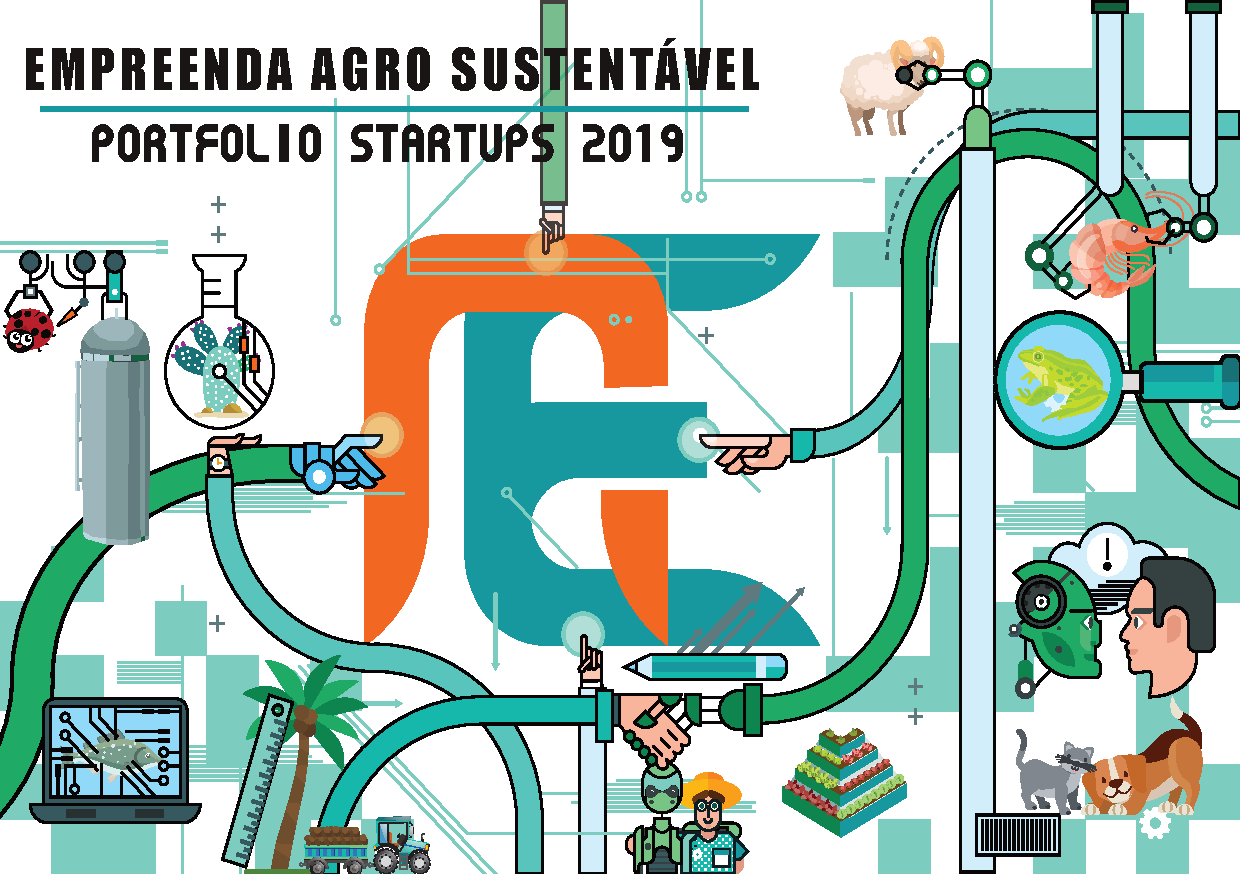
\includegraphics[scale=1.6]{Imagens/portfolio.png}
\fonte{Autoria própria}
\label{figura_12}
\end{figure}

\newpage

\subsection{Aqua plant}


Atualmente é destinado a irrigação cerca de 73\% da água potável consumida no mundo.  No entanto, nós sabemos que nem todas as regiões dispõem desse recurso, por exemplo, em 2019, 88,61\% da área do Nordeste foi afetada pela seca, com 2551 eventos de seca, de acordo com a \citeonline{ana_serie_2015}, isso afeta diretamente aqueles que dependem de sua produção para sustentar sua família. É muito ruim não ter certeza do amanhã, não acha?! Pior ainda é ter suas esperanças frustradas, e é isso  que geralmente acontece com produtores de regiões semiáridas, eles não sabem se naquele ano vai chover o suficiente e se não chove a plantação  não vinga, e esse fato reflete diretamente nos cofres do Governo Federal  que gasta em média 9 bilhões em investimentos no combate á seca (em medidas como Garantia-safra e Bolsa Estiagem).

\textbf{MODELO DO NEGÓCIO}

A Startup visa justamente acabar com as incertezas que  afligem o agricultor quanto á sua produção, visto que nosso produto é um sistema de aquaponia fechado, com recirculação de água, ao qual no final do processo o produtor terá garantido proteína e hortaliças de qualidade. Nós venderemos nosso produto, que irá integrado em pacotes de assistência técnica, tanto diretamente ao produtor como também em contratos com municípios. Nossa equipe é formada por 3 estudantes de Engenharia Agronômica e 2 Engenheiros de pesca, e por meio desse ciclo a AquaPlant irá fazer produzir no Sertão.


\begin{figure}[!htb]
\centering
\caption{\textbf{Marca Aquaplant}}
\includegraphics[scale=0.4]{Imagens/aquaplant.png}
\fonte{\cite{ufs_empreenda_2019-1}}
\label{figura_13}
\end{figure}
\newpage

\subsection{Agrion}

Dificuldade na relação entre os consumidores. Para os produtores existe a dificuldade no escoamento dos produtos devido a baixo poder de negociação com o atravessador e também como a ausência  de divulgação dos produtos. Já o cliente final sofre com o elevado preços e má qualidade dos produtos, e também dificuldade na rastreabilidade e proveniência dos produtos agropecuários.

\textbf{MODELO DE NEGÓCIO}

Aplicativo desenvolvido por sistemas digitais afim de conectar diretamente os aplicativos desenvolvido para sistemas produtores aos mercados varejistas no processo de compra e venda de produtos agrícolas onde a lucratividade é prevista por meio da cobrança de taxação em cima do montante total de vendas diferenciando valores de venda em atacado e varejo, e porcentagem por tipo de produto.

\textbf{TAMANHO DO MERCADO}

O grande número de produtores agrícolas  do mercado sergipano com relativo que  em sua grande maioria são oriundos da agricultura familiar e ao mesmo tempo um contingente potencial de consumidores em uma curta distância. Isso baseado na  participação das cooperativas desses produtos que de acordo 
com federação tem mais de 75 cooperados e que, as mesmas têm demostrado ter capacidade de suprir o aumento da demanda.


\begin{figure}[!htb]
\centering
\caption{\textbf{Marca Agrion}}
\includegraphics[scale=0.2]{Imagens/agrion.png}
\fonte{\cite{ufs_empreenda_2019-1}}
\label{figura_14}
\end{figure}
\newpage

\subsection{BAgrotec}

\textbf{PROBLEMA}

Você sabia que a produção está relacionada a uma boa assistência técnica realizada por um profissional capacitado? Imagine quanto de produção se perde no campo por falta de uma assistência técnica? E quantos profissionais estão sofrendo com o mercado competitivo se deslocando da sua área de Formação, muitas vezes porque a oportunidade não foi ofertada. 

\textbf{PROPOSTA}

Com o App TecAgro iremos conectar o produtor ao profissional, solucionando problemas no campo e consequentemente, gerando mercado de trabalho para os profissionais. Além do app o site da BAgroTec irá auxiliar no cadastramento de produtores que tiverem dificuldades com a plataforma mobile.  

\textbf{DIFERENCIAL DO NEGÓCIO}

O aplicativo irá valorizar o profissional gerando currículo dentro da plataforma  produtor terá acesso e retorno Imediato do profissional. Irá e fornecerá dados que irá auxiliar o profissional na tomada de decisão no campo

\textbf{POR QUE INVESTIR NO BAgrotec?}

Muito mais que ofertar serviços de assistência técnica estamos ofertando qualidade na produção e mudaremos o atual cenário da desvalorização do profissional das agrárias.

\begin{figure}[!htb]
\centering
\caption{\textbf{Marca BAgrotec}}
\includegraphics[scale=1.0]{Imagens/bagrotec.png}
\fonte{\cite{ufs_empreenda_2019-1}}
\label{figura_15}
\end{figure}
\newpage


\subsection{AGROPEC}


\textbf{PROBLEMA}

Você sabia que o Brasil tem um grande potencial para a produção de carne de cordeiro? Pois é, e mesmo assim não consegue suprir 
sua demanda interna. Segundo UFPR no ano de 2017 o Brasil importou 7.000 toneladas de carne de cordeiro. O valor praticado pelo mercado mostra a superioridade da carne de cordeiro, de acordo com a Embrapa, no mês de setembro o preço pago pelo kg/vivo do cordeiro em São Paulo foi de 8,83 reais, isso representa um valor 34,4\% a mais que a carne 
bovina. Contudo, para acessar esse mercado é necessário padronizar o produto e produzir em escala. No outro extremo da cadeia produtiva temos fazendas que possuem capacidade de produção, mas não o fazem por falta de assessoramento técnico e desconexão com os canais  de comercialização de cordeiros acabados, de matrizes e reprodutores.

\textbf{PROPOSTA}

A proposta da Startup, é aproximar a indústria frigorifica dos  produtores rurais, gerindo os rebanhos, administrando um 
confinamento coletivo, comercializando animais terminados para os frigoríficos e vendendo matrizes e reprodutores em plataformas de vendas online. Iniciaremos o trabalho com 10 fazendas e um rebanho geral de 1000 matrizes, sendo planejado triplicar o rebanho atendido até o final do sétimo ano e faturar anualmente pouco mais de dois milhões de reais.

\textbf{MODELO DE NEGÓCIO}

O modelo de negócio está baseado na produção de carne de  cordeiro com eficiência zootécnica e na gestão financeira, além 
da bonificação dos resultados, compra e venda de produtos  agrícolas onde a lucratividade é prevista por meio da cobrança de taxação em cima do montante total de vendas diferenciando valores de venda em atacado e varejo, e porcentagem por tipo de produto.


\begin{figure}[!htb]
\centering
\caption{\textbf{Marca AGROPEC}}
\includegraphics[scale=0.2]{Imagens/agropec.jpg}
\fonte{\cite{ufs_empreenda_2019-1}}
\label{figura_15}
\end{figure}
\newpage

\subsection{Agro View}

\textbf{PROBLEMA}

A startup de aplicações dos defensivos agrícolas nas grandes lavouras. Agroview, busca soluções que possam diminuir o número 
Visto que o uso indiscriminado   tem causado grandes prejuízos aos produtores, contaminação do meio ambiente, intoxicação dos animais e da população através de resíduos de agrotóxico nós alimentos. Segundo pesquisa da Anvisa (Agência Nacional de Vigilância Sanitária) os alimentos mais consumidos pela população brasileira: frutas, verduras, legumes e cereais, estão com a quantidade de resíduos de agrotóxico maior que os valores permitidos. Na Europa esses valores permitidos chegam a ser 5.000 vezes menor que no Brasil, devido a isso, os Europeus 
estão cada vez mais exigentes, obrigando o Brasil a produzir alimentos mais com mais qualidade e segurança. Desse modo, a Agroview busca minimizar o número de aplicações dos defensivos agrícolas, nas grandes lavouras, com uso do controle biológico das pragas e doenças, usando inimigos naturais.

\textbf{PROPOSTA}

Os Agroview, para terem um monitoramento mais intensivo da  produção terão que fazer um contrato mensal com a 
sua lavoura, afim de ser mais assertivo na identificação e tomada de decisão de aplicar os produtos  na hora certa, controlando antes que as pragas possam causar danos severos a lavoura, e assim  evitando uso desnecessário dos agrotóxicos. O controle quando necessário, será realizado com o uso de um drone, para dar mais agilidade ao processo e eficiência principalmente em local de difícil acesso, onde pessoas e até máquinas conseguiriam chegar, caso  de áreas muito declivosas. Essa empresa é composta por três engenheiros Agrônomos e um Engenheiro Agrícola, preparados para fazer controle biológico, seguindo  essa  visão sustentável que  já é uma tendência global. Temos um mercado gigante e promissor a ser  conquistado não só no Brasil, mas também no mundo inteiro.

\textbf{MODELO DE NEGÓCIO}

Onde a startup irá disponibilizar todos os nossos serviços e  osso modelo de negócio é baseado em assinaturas mensais assistência técnica ao produtor rural. E também contratos emergenciais. Ademais, nosso cliente pode entrar em contando por meio de telefone celular e redes sociais.


\begin{figure}[!htb]
\centering
\caption{\textbf{Marca Agro View}}
\includegraphics[scale=0.2]{Imagens/agroview.jpg}
\fonte{\cite{ufs_empreenda_2019-1}}
\label{figura_19}
\end{figure}


\subsection{Be Soluções}

No atual cenário global, há cada vez uma maior demanda por métodos produtivos mais sustentáveis, especialmente quando relacionados a recursos hídricos. De acordo com a Agência Nacional de Águas (ANA), o Brasil está entre os dez países com a maior área irrigada, com cerca de 6,95 milhões de hectares (Mha), que produzem alimentos utilizando diferentes técnicas de irrigação. Segundo o Sistema Nacional de Informações sobre o Saneamento (SNIS), calcula-se que no Brasil o consumo médio de água é de 10,4 trilhões de litros ao ano, onde deste total, pouco mais de 7 trilhões são destinados à agricultura, e que deste 7 trilhões destinado a este setor, aproximadamente 3 trilhões são desperdiçados devido ao mau uso.
\textbf{PROPOSTA}
Para reduzir essa problemática propomos a utilização de um sistema. Um pacote tecnológico com sensores instalados em campo, que coletam dados importantes como: umidade, temperatura e condutividade elétrica, tudo em tempo real, que serão transmitidos sem fio para uma central eletrônica para um controle preciso do sistema
de irrigação, permitindo o uso mais eficiente e sustentável dos recursos hídricos.
\textbf{CLIENTES}
Para reduzir essa problemática propomos a utilização de um sistema. Um pacote tecnológico com sensores instalados em campo, que coletam dados importantes como: umidade, temperatura e condutividade elétrica, tudo em tempo real, que serão transmitidos sem fio para uma central eletrônica para um controle preciso do sistema de irrigação, permitindo o uso mais eficiente e sustentável dos recursos hídricos.

\textbf{DIFERENCIAL}
Diferente dos sistemas atuais que possuem um alto custo e que não apresentam tantos recursos de forma unificada em um só equipamento, buscamos desenvolver um produto que proporcione uma alta precisão ao utilizar um sistema de dados coletados em tempo real, obtidos no local especifico da cultura. Esse equipamento é adaptativo as diferentes culturas e tipos de solo. Através de uma simples configuração na central eletrônica, por meio de uma de tela \textbf{touch} e interface intuitiva, é possível realizar uma irrigação precisa com somente a quantidade de água que a cultura selecionada necessite.

\begin{figure}[!htb]
\centering
\caption{\textbf{Marca Be Soluções}}
\includegraphics[scale=0.4]{Imagens/besolucoes.png}
\fonte{\cite{ufs_empreenda_2019-1}}
\label{figura_20}
\end{figure}




\subsection{Grão Nordestino}

\textbf{PROBLEMA}

Tendo em vista que bilhões de pessoas passam fome em nosso país e no mundo, nós da startup Grão Nordestino temos como principal objetivo o combate ao desperdício de alimentos, uma vez que cerca 1/3 de todo alimento produzido é desperdiçado. Essas perdas seriam suficientes para alimentar 2 bilhões de pessoas e 54\% desse desperdício vem da produção.

\textbf{PROPOSTA}

Conhecendo a realidade do pequeno e médio produtor que por falta de uma unidade armazenadora perdem boa parte da sua colheita ou são obrigados a vender com o menor preço para que não venha a perder seu produto, nós da grão Nordestino trazemos o que vem a ser a solução para esse problema, projetando e instalando silos de baixo custo e sustentáveis, agregando valor ao seu produto e combatendo o desperdício de alimentos mal armazenados.

\textbf{DIFERENCIAL DO NEGÓCIO}

O produtor terá acesso e retorno Imediato do profissional, irá valorizar o profissional gerando currículo dentro da plataforma e fornecerá dados que irá auxiliar o profissional na tomada de decisão no campo.


\begin{figure}[!htb]
\centering
\caption{\textbf{Marca Grão Nordestino}}
\includegraphics[scale=0.3]{Imagens/graonordestino.png}
\fonte{\cite{ufs_empreenda_2019-1}}
\label{figura_21}
\end{figure}
\newpage



\subsection{Horta House}

\textbf{PROBLEMA}

Segundo a ONU o Brasil possui hoje uma taxa de urbanização equivalente a 85\%, sendo estimado no último relatório que esse número irá atingir 90\% em 2020, isso faz com que cada vez mais as pessoas se agrupem em moradias com espaços limitados e com difícil acesso a áreas que lhe permitam cultivar alguns alimentos e até plantas ornamentais.

\textbf{PROPOSTA}

Tendo em vista esse problema algumas soluções têm sido empregadas e crescido de forma exponencial nos últimos anos. Algumas dessas soluções são a construção de hortas comunitárias em condomínios e hortas individuais em apartamentos, algumas construídas pelas próprias construtoras. Mas surge um questionamento muito comum entre as pessoas que as utilizam, como plantar?
O número de empresas especializadas em consultoria para hortas urbanas ainda é insuficiente para atender essa demanda que continua a crescer, tentando solucionar esse problema muitas pessoas recorrem a ferramentas de busca na internet e acabam tomando como base instruções de pessoas que muitas vezes não possuem uma qualificação para recomendações técnicas, o que em alguns casos acaba fazendo com que as plantas cultivadas entrem em um processo inverso ao desejado, ou seja morrem!

\textbf{DIFERENCIAL DO NEGÓCIO}

Visando solucionar esses problemas nossa empresa pretende fornecer consultoria técnica de qualidade, tendo em vista que nossa equipe é formada por três engenheiros agrônomos. Junto a nossa
consultoria pretendemos ofertar a construção de hortas planejadas de forma a que as mesmas se adéquem as necessidades do cliente, sendo incluído nesse planejamento o fornecimento de substrato, soluções nutritivas e adubos orgânicos, além das mudas.


\begin{figure}[!htb]
\centering
\caption{\textbf{Marca Horta House}}
\includegraphics[scale=0.1]{Imagens/hortahouse.png}
\fonte{\cite{ufs_empreenda_2019-1}}
\label{figura_21}
\end{figure}
\newpage


\subsection{ItecAgro}

Plataforma de interação direta com uma equipe multidisciplinar voltada
para o agro, que se utiliza de sistemas digitais para dinamizar seu
negócio de forma: Inovadora, Empreendedora e Sustentável;

\textbf{MISSÃO}

Propor um canal facilitador, através de sistemas digitais para dinamizar o negócio da agricultura de forma inovadora, empreendedora, e sustentável.

\textbf{VISÃO}

Ser uma startup de referência desenvolvendo soluções através da assistência técnica de qualidade gerando valor ao produtor e promovendo responsabilidade socioambiental, e trabalho com excelência.

\textbf{VALORES}
Inovação, Humanização, Sustentabilidade, Ética, Transparência, Profissionalismo, Confiabilidade e Tecnologia.

\begin{figure}[!htb]
\centering
\caption{\textbf{Marca Itec Agro}}
\includegraphics[scale=0.1]{Imagens/itecagro.png}
\fonte{\cite{ufs_empreenda_2019-1}}
\label{figura_22}
\end{figure}
\newpage


\subsection{Impacto Pescados}

\textbf{CARACTERÍSTICA DO NEGÓCIO}

Empresa especializada na criação de camarão do tipo \textit{Litopenaeus vannamei} com a utilização de bomba movida a óleo diesel para sucção da água do mar viabilizando as trocas de água com uma maior frequência tornando o menor tempo de cultura lançando no mercado um produto de qualidade com um menor período de cultivo. Em outras palavras baixamos o tempo de cultivo para 30 dias. A despesca do camarão de 10 gramas. O cultivo pesquisado num criador comum, foram necessários 70 dias para mesma gramatura. Custa-se, dessa forma, 5,00R\$kg do camarão cinza. Podendo, assim, vender o produto a 15,00R\$ no mínimo. Segundo a Embrapa a pesca mundial não supre a demanda por pescados, ou seja, há um problema no equilíbrio entre a oferta e a demanda. Além disso, existe o fato do preço elevado para o camarão. Sendo assim, soluciona-se esta problemática com criação de camarão em viveiros além de fazê-lo com o menor preço e melhor atendimento.

\textbf{PROPOSTA}

Visto isso, nota-se que nosso lucro gira em torno de 200\% a cada 30 dias no Máximo, o qual é no modo monofásico-quando com apenas um tanque, você faz as fases: pré-berçário, berçário e engorda. Aliado a isso podemos fazer no modo trifásico conforme o capital disponível para custear três tanques pra fazer as três fases e diminuir a 11 dias a despesca.

\begin{figure}[!htb]
\centering
\caption{\textbf{Marca Impacto Pescados}}
\includegraphics[scale=0.4]{Imagens/imacto_pescados.jpg}
\fonte{\cite{ufs_empreenda_2019-1}}
\label{figura_23}
\end{figure}
\newpage


\subsection{La Flora Pet}

\textbf{PROBLEMA}

Observando o crescimento do mercado PET nos últimos anos e a persistência nas dores sofridas pelos donos desses animais com relação a custo alto e acessibilidade a tratamentos eficientes, a La Flora Pet desenvolve produtos naturais e artesanais com base em extratos ou óleos essenciais cujo objetivo é prevenir ou tratar distúrbios comportamentais e dermatológicos em cães e gatos ofertando produtos de baixo custo

\textbf{PROPOSTA}

Sabendo das limitações variadas de cada espécie, raça, idade e sexo do animal, nossos profissionais são capacitados a atender de forma intimista a necessidade do usuário sem causar transtornos toxicológicos e agindo de forma eficiente no tratamento ou prevenção de doenças. La Flora Pet a magia da natureza a um clique de distância.

\textbf{DIFERENCIAL DO NEGÓCIO} 

Nosso plano de negócio é a venda desses produtos, que através do site da loja será personalizado pelo próprio cliente. Após cadastramento de dados pessoais do cliente e usuário, a personalização consiste em escolher o extrato ou óleo essencial de acordo a finalidade terapêutica desejada, o formato, a cor e o tamanho do produto, constatadas essas informações será solicitado e após fabricação seguirá para o endereço do cliente.


\begin{figure}[!htb]
\centering
\caption{\textbf{Marca La Flora pet}}
\includegraphics[scale=4.5]{Imagens/laflorapet.png}
\fonte{\cite{ufs_empreenda_2019-1}}
\label{figura_24}
\end{figure}
\newpage




\subsection{MAMP}

\textbf{PRODUTO}

Mas por que a palma? A Palma é um símbolo de resistência do Nordeste, sendo também um alimento considerados pancs: plantas alimentícias não-convencionais. A palma não é um alimento convencional no Brasil, porém lá no México e em outros países com influência mexicana já existem mais de 200 receitas utilizando ela. O que torna o mercado muito amplo e com diversas oportunidades. Ela é totalmente nutritiva, rica em proteínas, fibras e um ótimo antioxidante e corante natural o que faz dela uma ótima opção de alimento rápido e saudável para acompanhar a correria do dia-a-dia.

\textbf{PROPOSTA}

Pensando nisso o nosso produto foi desenvolvido principalmente para o público Fitness e vegetarianos. O mercado Fitness tem uma grande demanda de uma alimentação saudável, por isso trouxemos a Palma como alternativa para suprir essa carência do mercado. Esse que atualmente são abastecidos com produtos de valor altíssimo, agregando ao nosso produto o baixo custo e alto lucro.

\textbf{DIFERENCIAL DO NEGÓCIO}

Nossa linha foi inteiramente pensada para acompanhar o slogan da marca: mamp é alimentar com o sabor do Nordeste. Por isso nossas embalagens sustentáveis e recicláveis trazem a rusticidade e beleza dessa região maravilhosa.



\begin{figure}[!htb]
\centering
\caption{\textbf{Marca MAMP}}
\includegraphics[scale=0.1]{Imagens/mamp.png}
\fonte{\cite{ufs_empreenda_2019-1}}
\label{figura_22}
\end{figure}
\newpage




\subsection{Ranagro}

\textbf{PROBLEMA}
Nós da Ranagro enxergamos algumas lacunas no processo de confinamento da rã- touro para abate, umas delas é a falta de uma ração específica que atenda às necessidades nutricionais do animal. A rã-touro é a única espécie utilizada por ranicultures brasileiros, uma vez que é a melhor opção para a criação intensiva, e tem uma adaptação perfeita com nossas condições climáticas. O mercado está cada vez mais competitivo, assim sendo necessário uma inovação para alcançar o resultado satisfatório e economicamente viável para o produtor e consumidor, além de trazer tecnologias inovadoras para o ramo da ranicultura. A qualidade e sustentabilidade é vista como uma arma de estratégia para a expansão da empresa. A carne de rã está sendo cada vez mais valorizada e consumida em restaurantes, no qual passou a ser recomendados por médicos e nutricionistas, pois sua taxa de gordura é de apenas três por cento, sendo a única carne produzida em cativeiros que possui dez aminoácidos e indicados também para alimentação de crianças que possuem rejeição à proteína animal, assim, podendo expandir cada vez mais seu consumo. A ração oferecida no mercado é mesma empregada na criação de peixes que acarreta um menor aproveitando da carne e elevando o custo para a engorda.

\textbf{PROPOSTA}

Assim a Ranagro, veio com uma proposta inovadora para o mercado que é a comercialização de uma ração específica, para haver um menor custo,menor impacto ambiental, crescimento rápido, boa lucratividade e um alto aproveitamento, no qual pode chegar muito próximo a cem por cento, se for considerado a exploração do mercado de subprodutos, como o fígado para pavê e a pele, que atende a medicina humana na recuperação de queimaduras. A ranicultura é uma nova oportunidade para ser explorada no agronegócio e a criação e comercialização da carne de rã, pode ser uma nova forma de ampliar o nicho agrário do país. Nosso grupo é formado por três graduastes de zootecnia e dois de engenharia agronômica, obrigada pela atenção de todos.



\begin{figure}[!htb]
\centering
\caption{\textbf{Marca Ranagro}}
\includegraphics[scale=0.7]{Imagens/ranagro.png}
\fonte{\cite{ufs_empreenda_2019-1}}
\label{figura_26}
\end{figure}
\newpage


\subsection{Tecno Coco}

\textbf{PROBLEMA}

Com a chegada do verão, a tendência é que haja um aumento do consumo da água de coco e consequentemente do volume de resíduo a ser descartado no meio ambiente. Considerando esta problemática, nós da Tecno Coco nos vimos motivados a buscar uma solução para este impacto ambiental. Os aterros sanitários sempre foram a solução de descarte. Porém no atual cenário, já não comportam mais essa demanda, tanto que foi criada uma lei municipal limitando a coleta em 200 kg por comerciante, o que gera um impacto ambiental considerável, pois os aterros absorvem aproximadamente 190 toneladas por semana. Então, além do que é destinado aos aterros, o que faremos com o excedente?

\textbf{PROPOSTA}

A ideia da Tecno Coco é gerar uma cadeia cíclica de produção onde o Campo produz o coco, que é destinado ao comerciante, vendido ao usuário onde é descartado e processada pela nossa Startup retornando ao Campo como insumo agrícola, auxiliando na produtividade. Outra parte será destinada a outras cadeias produtivas e manufaturas, como material para isolamento acústico, reforço de materiais, enchimento de estofados, mantas para proteção do solo e muitos outros produtos que esse resíduo pode ser transformado.

\textbf{DIFERENCIAL DO NEGÓCIO}

Uma startup que está em fase de desenvolvimento por alunos da Universidade Federal de Sergipe e que tem como objetivo resolver o problema ambiental gerado pelo o acumulo de resíduos do coc o no nosso estado.

\begin{figure}[!htb]
\centering
\caption{\textbf{Marca Tecno Coco}}
\includegraphics[scale=2.0]{Imagens/tecnococo.png}
\fonte{\cite{ufs_empreenda_2019-1}}
\label{figura_27}
\end{figure}
\newpage


\subsection{Une Agro}

\textbf{PROBLEMA}

Imagine se uma fabrica produzisse uma produto que o único escoamento dele fosse para uma distribuidora na região, essa distribuidora ia ditar preço e quantidade que iria comprar os produtos, podendo até perder a produção. Qual incentivo essa fabrica teria de produzir? Bem isso acontece com diversos agricultores no Brasil, ficam refém apenas de um atravessador que vai até a porta dele para escoar seus produtos, sendo que o atravessador fica com maior parte dos lucros, e muitas vezes o que paga a agricultor é só o custo da produção.

\textbf{PROPOSTA}

A UneAgro pensando nisso, elaboramos um aplicativo onde o produtor possa anunciar seus produtos de forma pratica e rápida, sem sair de casa, onde ele irá ter uma amplo leque de clientes que estão interessados no produto dele.

\textbf{DIFERENCIAL DO NEGÓCIO}

O aplicativo é desenvolvido para as duas personas, tanto para agricultor quanto para o distribuidor, pois o distribuidor também sai ganhando ao utilizar o aplicativo pois terá uma maior quantidade localidade e preços pelo mesmo produto, podendo negociar com todas. O aplicativo será totalmente gratuito, sendo que a receita da empresa se originará nas parcerias anunciantes e seus produtos no aplicativo, além de disponibilizar informações produtos que serão disponibilizados para os usuários através de um pacote mensal ou anual, onde esses info-produtos estarão relacionados ao próprio desenvolvimento de negócio dos usuários, como aulas e \textit{podcasts} sobre gestão e produção agrícola.

\begin{figure}[!htb]
\centering
\caption{\textbf{Marca Une Agro}}
\includegraphics[scale=1.5]{Imagens/uneagro.png}
\fonte{\cite{ufs_empreenda_2019-1}}
\label{figura_28}
\end{figure}
\newpage

